\subsection{Cost of coupling}\label{sec:eval:micro}

All timings in this section come from one process pinned to one core of the server while nothing else runs; each value
is the median of seven timed calls after a warm-up, and the median over three repetitions.

\paragraph{Queries.} Batching is what makes shared models cheap (Fig.~\ref{fig:micro-queries}). A single surface-height
lookup costs 21.8\,$\mu$s, almost all of it call overhead; in batches of 10,000 it costs 0.01\,$\mu$s per point. The
corridor top along a return line, the query F1 needs, costs 63.6\,$\mu$s per line with an exact cell traversal and
0.61\,$\mu$s per line on the max-pooled height pyramid in batches of 1,000, a factor of 104. A line-of-sight test costs
9.8\,$\mu$s per pair in the maximal batch of 64. The environment field shows the same pattern: a wind query costs
27.8\,$\mu$s when issued point by point and 0.16\,$\mu$s per point in a batch of 10,000, and a slant optical depth
0.04\,$\mu$s per path. Evaluating all fields at once costs only a quarter more than wind alone, so a decision that
needs wind, visibility and density pays for one query, not three.

\begin{figure}[t]
\centering
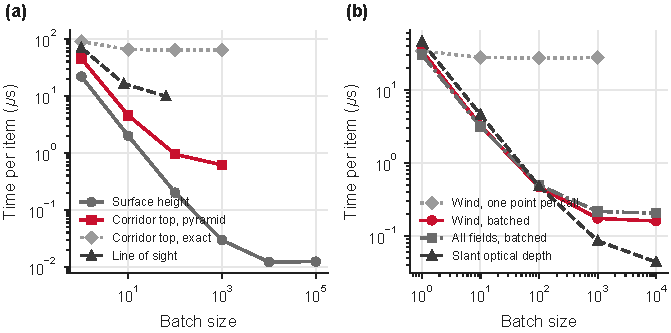
\includegraphics[width=\textwidth]{figures/pdf/micro_queries.pdf}
\caption{Query cost per item against batch size. (a) Geometry service: surface height, corridor top along a line (exact
traversal and pyramid sampling) and line of sight. (b) Environment field: wind one point per call and batched, all
fields batched, and slant optical depth}
\label{fig:micro-queries}
\end{figure}

\paragraph{Return refresh.} The rotating schedule turns the impossible schedule of F4 into a negligible one
(Fig.~\ref{fig:m4}). At 1,000 drones each 5\,Hz call refreshes 200 plans in 0.25\,ms, which amounts to 1.25
core-milliseconds per simulated second, against 3.1 for refreshing every drone at 5\,Hz, 153 for refreshing every drone
at every tick and 13,400 for doing so with exact corridors. The cost grows by a factor of 1.7 from 10 to 1,000 drones
because the fixed per-call overhead dominates; it stays below the 2 core-milliseconds the return stage is budgeted.
Plans are at most one second old, which at 3--8\,m/s is 3--8\,m of travel, well inside the 10\,m safety margin of the
clearance envelope.

\paragraph{Whole pipeline.} Figure~\ref{fig:micro-stages} runs the complete runtime with $N$ drones in rain, nearly
all flying, for 20 simulated seconds: environment, dynamics and control, sensors, contact and separation, the safety
state machines with the battery and return logic, missions and state publication, at the 4\,ms tick; scan planning and
delegation are invoked on demand and timed separately below. On a single core the runtime advances 1,000 drones at \STAGERTF{} times real time, so
real time needs \STAGECORE{} core-seconds per simulated second, inside the 0.40 budget; with 10 drones it runs
\STAGERTFTEN{} times faster than real time. Of the \STGTOT{} core-milliseconds the stages use per simulated second at
1,000 drones (\STGWALL{} including the loop around them), safety and energy take \STGSAFE{}, dynamics and control
\STGDYN{}, missions \STGMIS{}, the environment \STGENV{} and state publication \STGPUB{}. The environment stage grows
only from \STGENVTEN{} to \STGENV{} core-milliseconds between 10 and 1,000 drones, because one batched query serves
the whole fleet; the coupled decisions are thus not what limits the fleet size.

\begin{figure}[t]
\centering
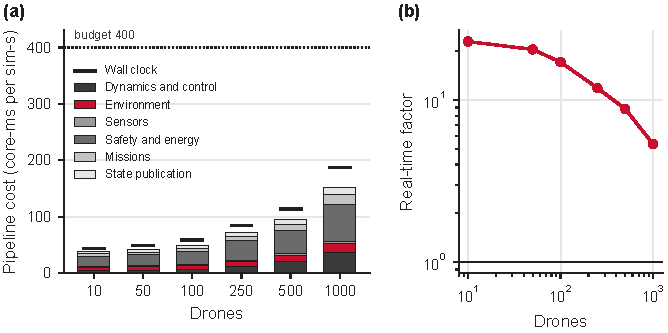
\includegraphics[width=\textwidth]{figures/pdf/micro_stages.pdf}
\caption{Whole pipeline with $N$ drones flying in rain, one core. (a) CPU cost per simulated second by stage group;
the dotted line is the 0.40 core-second budget. (b) Real-time factor (simulated seconds per wall-clock second)}
\label{fig:micro-stages}
\end{figure}

% \paragraph{Scan planner.} The perception-driven scan planner of Sect.~\ref{sec:design:decisions} plans a 0.04\,km$^2$
% area in 0.3\,s and a 4\,km$^2$ area in 2.0--2.4\,s (Fig.~\ref{fig:micro-coverage}), roughly linear in area. Planning therefore takes
% seconds, while the scans it plans take tens of minutes, and it can be rerun whenever the weather changes.

% \begin{figure}[t]
% \centering
% 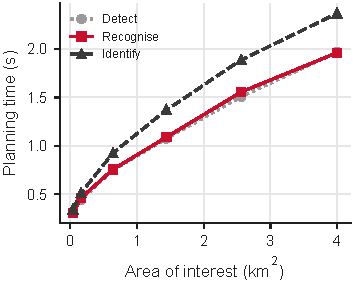
\includegraphics[width=0.55\textwidth]{figures/pdf/micro_coverage.pdf}
% \caption{Scan-planner runtime against the area of interest, per required perception level; median of three
% repetitions}
% \label{fig:micro-coverage}
% \end{figure}
